\documentclass[hidelinks,12pt]{article}
\usepackage[left=0.25cm,top=1cm,right=0.25cm,bottom=1cm]{geometry}
%\usepackage[landscape]{geometry}
\textwidth = 20cm
\hoffset = -1cm
\usepackage[utf8]{inputenc}
\usepackage[spanish,es-tabla]{babel}
\usepackage[autostyle,spanish=mexican]{csquotes}
\usepackage[tbtags]{amsmath}
\usepackage{nccmath}
\usepackage{amsthm}
\usepackage{amssymb}
\usepackage{mathrsfs}
\usepackage{graphicx}
\usepackage{subfig}
\usepackage{standalone}
\usepackage[outdir=./Imagenes/]{epstopdf}
\usepackage{siunitx}
\usepackage{physics}
\usepackage{color}
\usepackage{float}
\usepackage{hyperref}
\usepackage{multicol}
%\usepackage{milista}
\usepackage{anyfontsize}
\usepackage{anysize}
%\usepackage{enumerate}
\usepackage[shortlabels]{enumitem}
\usepackage{capt-of}
\usepackage{bm}
\usepackage{relsize}
\usepackage{placeins}
\usepackage{empheq}
\usepackage{cancel}
\usepackage{wrapfig}
\usepackage[flushleft]{threeparttable}
\usepackage{makecell}
\usepackage{fancyhdr}
\usepackage{tikz}
\usepackage{bigints}
\usepackage{scalerel}
\usepackage{pgfplots}
\usepackage{pdflscape}
\pgfplotsset{compat=1.16}
\spanishdecimal{.}
\renewcommand{\baselinestretch}{1.5} 
\renewcommand\labelenumii{\theenumi.{\arabic{enumii}})}
\newcommand{\ptilde}[1]{\ensuremath{{#1}^{\prime}}}
\newcommand{\stilde}[1]{\ensuremath{{#1}^{\prime \prime}}}
\newcommand{\ttilde}[1]{\ensuremath{{#1}^{\prime \prime \prime}}}
\newcommand{\ntilde}[2]{\ensuremath{{#1}^{(#2)}}}

\newtheorem{defi}{{\it Definición}}[section]
\newtheorem{teo}{{\it Teorema}}[section]
\newtheorem{ejemplo}{{\it Ejemplo}}[section]
\newtheorem{propiedad}{{\it Propiedad}}[section]
\newtheorem{lema}{{\it Lema}}[section]
\newtheorem{cor}{Corolario}
\newtheorem{ejer}{Ejercicio}[section]

\newlist{milista}{enumerate}{2}
\setlist[milista,1]{label=\arabic*)}
\setlist[milista,2]{label=\arabic{milistai}.\arabic*)}
\newlength{\depthofsumsign}
\setlength{\depthofsumsign}{\depthof{$\sum$}}
\newcommand{\nsum}[1][1.4]{% only for \displaystyle
    \mathop{%
        \raisebox
            {-#1\depthofsumsign+1\depthofsumsign}
            {\scalebox
                {#1}
                {$\displaystyle\sum$}%
            }
    }
}
\def\scaleint#1{\vcenter{\hbox{\scaleto[3ex]{\displaystyle\int}{#1}}}}
\def\bs{\mkern-12mu}


\usepackage{apacite}
\title{Breviario de geometría diferencial \\ \large{Material de consulta previo}\vspace{-3ex}}
\author{M. en C. Gustavo Contreras Mayén}
\date{ }
\begin{document}
\vspace{-4cm}
\maketitle
\fontsize{14}{14}\selectfont
\tableofcontents
\newpage

\section{Introducción.}

En nuestra formación como físicos, hemos estudiado las curvas: cómo la curva giraba en un plano, y quizá en el espacio. Pasamos ahora a las superficies, que son objetos bidimensionales en un espacio tridimensional, encontramos entonces que el concepto de curvatura se traduce en superficies.
\par
En los cursos de cálculo, sabemos que las superficies se definen como gráficas de funciones de valor real de dos variables $z = f (x, y)$. Esta función también puede tomar la forma $x = f (y, z)$ o $y = f (x, z)$. En algunos casos, por otro lado, esta función se da implícitamente como $F (x, y, z) = 0$. Por ejemplo, una esfera de radio $a$ está dada por la expresión $x^{2} + y^{2} + z^{2} = a^{2}$ y es imposible obtener una sola función de dos variables que describa una esfera completa. Un cilindro $x^{2} + y^{2} = a^{2}$ es otro claro ejemplo. 

\section{Superficies.}
\subsection{El plano.}

La ecuación general de un plano es:
\begin{align*}
a \, x + b \, y + c \, z + d = 0
\end{align*}
Un plano está determinado de manera única a partir de un punto en él y un vector perpendicular al mismo plano, como se muestra en la figura (\ref{fig:figura_01_plano}).
\begin{figure}[H]
    \centering
    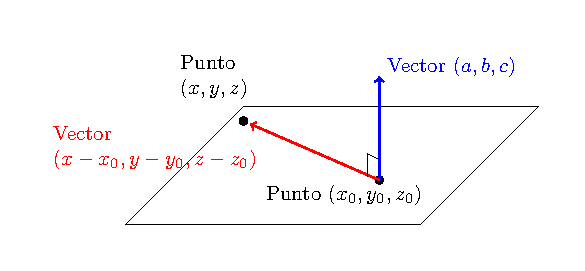
\includegraphics[scale=1.3]{Imagenes/Superficies_01_Plano.eps}
    \caption{Plano $a(x - x_{0}) + b(y - y_{0}) + c(z -z_{0}) = 0$}
    \label{fig:figura_01_plano}
\end{figure}

La ecuación que describe cualquier punto $ \vb{x} = (x, y, z)$ en el plano, mediante el punto $\vb{x}_{0} = (x_{0}, y_{0}, z_{0})$ perpendicular al vector $\vb{a} = (a, b, c)$ es:
\begin{align*}
\vb{a} \cdot (\vb{x} - \vb{x}_{0}) = 0
\end{align*}
La ecuación anterior del plano se puede expresar en su forma escalar como:
\begin{align*}
a \, (x - x_{0}) + b \, (y - y_{0}) + c \, (z -z_{0}) = 0
\end{align*}

\subsection{Superficies de revolución.}

Definimos $z = f(\sqrt{x^{2} + y^{2})}$, para obtener una representación esta superficie, graficamos la función $z = f(y)$ en el plano $y-z$ y la rotamos  alrededor del eje $z$.
\par
Por ejemplo:
\begin{itemize}
\item Un cono $z = a \, \sqrt{x^{2} + y^{2}}$ se obtiene rotando la línea $z = a \, y$.
\item Un paraboloide $z = a \, x^{2} + a \, y^{2}$ se obtiene al rotar la parábola $z = a \, y^{2}$.
\item Un hemisferio $z = \sqrt{a^{2} - x^{2} - y^{2}}$ se obtiene al rotar el semicírculo $z = \sqrt{a^{2} -y^{2}}$
\end{itemize}

\begin{figure}[H]%
\centering
\subfloat[][Cono]{{ 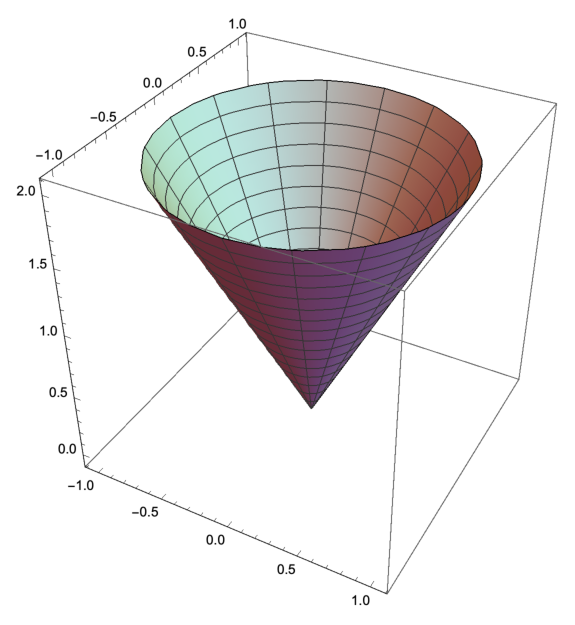
\includegraphics[scale=0.4]{Imagenes/Superficies_02_Cono.eps} }}%
\qquad
\subfloat[][Paraboloide]{{ 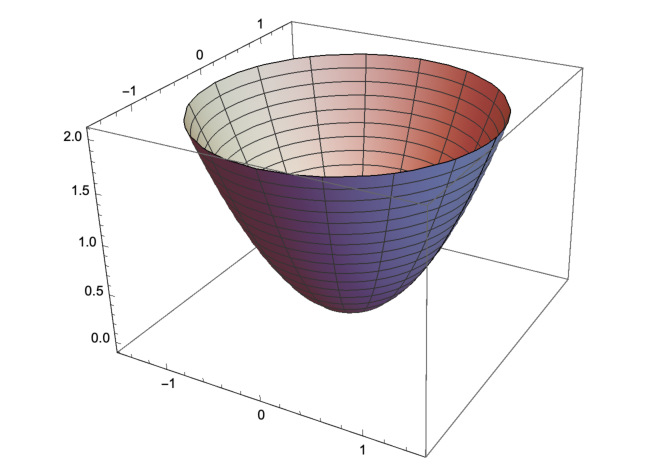
\includegraphics[scale=0.4]{Imagenes/Superficies_03_Paraboloide.eps} }}%
\qquad
\subfloat[][Hemisferio]{{ 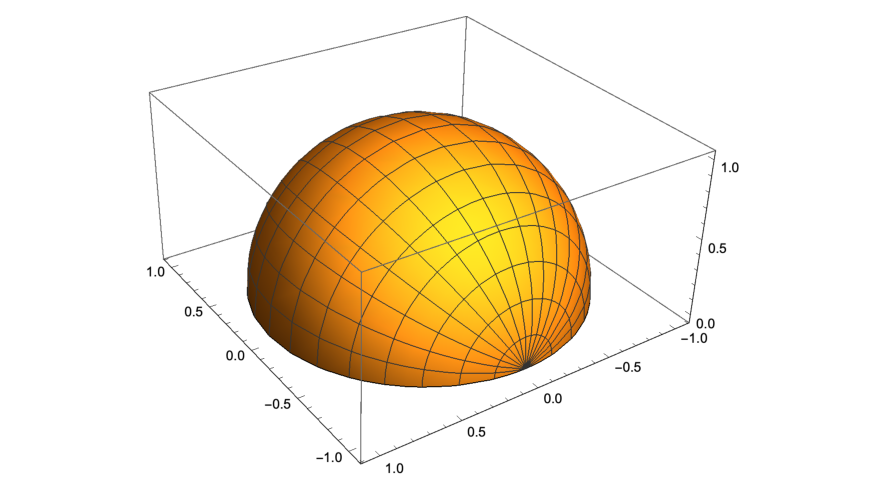
\includegraphics[scale=0.4]{Imagenes/Superficies_04_Hemisferio.eps} }}%
\caption{Superficies de revolución}%
\label{fig:example}%
\end{figure}

\subsection{Superficies paramétricas.}

En los casos en que una superficie se da como función implícita $F (x, y, z) = 0$, puede ser de utilidad describir las tres variables $x, y y z$ pero utilizando otros parámetros $u$ y $v$. En ese caso, se tiene que:
\begin{align*}
x = x (u, v) \hspace{0.5cm} y = y (u, v) \hspace{0.5cm} z = z (u, v)
\end{align*}
Estas ecuaciones se denominan \emph{ecuaciones paramétricas} de la superficie y la superficie dada mediante las ecuaciones paramétricas, se le denomina \emph{superficie paramétrica}.
\par
Por lo tanto, una superficie paramétrica se representa como una función vectorial de dos variables, es decir, el dominio $D$ consta de todos los valores posibles de los parámetros $u$ y $v$ que están en $\mathbb{R}^{2}$. El rango de las superficies está contenido en el espacio tridimensional $\mathbb{R}^{3}$.
\par
Por tanto, una superficie $\vb{x}$ es un mapeo de $D$ en $\mathbb{R}^{3}$. Esto se denota por $x: D \to \mathbb{R}^{3}$. La función vectorial $\vb{x}$ también se puede representar como:
\begin{align*}
\vb{x} (u, v) = (x (u, v), y (u, v), z (u, v))
\end{align*}
Observa una analogía con las curvas: podemos pensar en las curvas como objetos unidimensionales en el espacio tridimensional y las superficies como objetos bidimensionales en el espacio tridimensional. Por tanto, una curva se puede describir utilizando un solo parámetro $t$. La superficie, por otro lado, se describe usando dos parámetros $u$ y $v$.
\begin{table}[H]
\centering
\begin{tabular}{|l | c | c | c | c |} \hline
& Mapeo & Dim. & Parám. & Ecuaciones \\ \hline
Curva & $\gamma: (a, b) \subseteq \mathbb{R} \to \mathbb{R}^{3}$ & $1$ & $t$ & $\gamma(t) = (x(t), y(t), z(t))$ \\ \hline
Superficie & $\vb{x}: D \subseteq \mathbb{R}^{2} \to \mathbb{R}^{3}$ & $2$ & $u, v$ & $\vb{x} (u, v) = (x(u, v), y(u, v), z(u, v))$ \\ \hline
\end{tabular}
\end{table}
La curva dada en la forma $z = f(y)$ siempre se puede parametrizar como $\vb{x} = (x, y, f(x, y))$. Por ejemplo, el plano $2 x + 3 y + z = 6$ se puede representar por $\vb{x} = (x, y, 6 - 2 x - 3 y)$.
\par
Algunas otras superficies requieren parametrizaciones más sofisticadas. De trabajo que ya hemos tenido previamente ya sea en los cursos de Mecánica o de Electromagnetismo, recordemos las reglas de transformación para un sistema coordenado cilíndrico.

\subsection*{Coordenadas cilíndricas.}

Para las reglas de transformación:
\begin{align*}
x = r \, \cos \theta, \hspace{0.5cm} y = r \, \sin \theta, \hspace{0.5cm} z = z
\end{align*}
Sabemos que en este sistema de coordenadas $x^{2} + y^{2} = r^{2}$. 
\par
En este sistema coordenado cilíndrico, podemos obtener la parametrización de los siguientes ejemplos:
\begin{enumerate}[label=\alph*)]
\item El paraboloide $z= x^{2} + y^{2}$ se puede expresar como $x = r \cos \theta$, $y = r \, \sin \theta$ y $z = r^{2}$, como $x^{2} + y^{2} = r^{2}$, en coordenadas cilíndricas $z = r^{2}$, por lo que la parametrización es:
\begin{align*}
\vb{x} = (r \, \cos \theta, r \, \sin \theta, r^{2})
\end{align*}
Para este mismo paraboloide, la parametrización también se puede expresar como $(x, y, x^{2}+ y^{2})$.
\item El cono $z = \sqrt{x^{2} + y^{2}}$ tiene una representación parametrizada $\vb{x} = (r \, \cos \theta, r \, \sin \theta, r)$.
\item El cilindro $x^{2} + y^{2} = 4$, es tal que el valor de $r$ es constante y vale $2$, por lo que los dos parámetros restantes $\theta$ y $z$, los usamos para representar este cilindro como $x = 2 \, \cos \theta$, $y = 2 \, \sin \theta$, $z = z$, que de manera breve lo escribimos como $vb{x} = (2 \, \cos \theta, y = 2 \, \sin \theta, z)$.
\end{enumerate}

\subsection{Plano tangente.}

Para una superficie paramétrica:
\begin{align*}
\vb{x} = [x(u, v), y(u, v), z(u, v)]
\end{align*}
las derivadas $\vb{x}_{u}$ y $\vb{x}_{v}$ son vectores en el plano tangente. Esto es, su producto vectorial:
\begin{align*}
\pdv{\vb{x}}{u} \times \pdv{\vb{x}}{v} = (x_{u}, y_{u}, z_{u}) \times (x_{v}, y_{v}, z_{v})
\end{align*}
es perpendicular al plano tangente, como se aprecia en la figura (\ref{fig:figura_02_plano_tangente})
\begin{figure}[H]
    \centering
    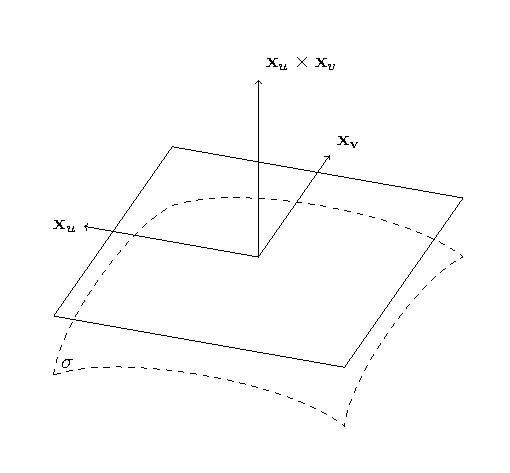
\includegraphics[scale=1]{Imagenes/Superficies_05_Plano_Tangente.eps}
    \caption{Superficie $\sigma$ y un plano tangente.}
    \label{fig:figura_02_plano_tangente}
\end{figure}

\section{Curvatura y el Teorema Egregium de Gauss.}

Para definir el concepto de curvatura de $\gamma$, es necesario que asegurar que es posible definir un vector tangente de longitud unitaria en cada punto. Esta condición se aseguró al exigir que la derivada $\dv*{\gamma}{t} \neq 0$.
\par
De manera análoga, para las superficies se requiere asegurar que el plano tangente en cada punto esté definido (es decir, que no esté colapsado en una línea o un punto). Dado que el vector normal al plano tangente de una superficie paramétrica $\vb{x}$ está dado por $\pdv{\vb{x}}{u} \times \pdv{\vb{x}}{v}$, queremos imponer una condición que garantice que este vector es distinto de cero, es decir:
\begin{align*}
\pdv{\vb{x}}{u} \times \pdv{\vb{x}}{v} \neq 0
\end{align*}

La condición anterior garantiza que los vectores $\pdv*{\vb{x}}{u}$ y $\pdv*{\vb{x}}{v}$ no están en la misma línea. Por lo tanto, son linealmente independientes y constituyen \emph{una base del plano tangente} y cualquier otro vector en el plano tangente se puede representar como una combinación lineal de estos dos vectores.
\par
Por lo tanto, consideraremos solo superficies tales que alrededor de cada punto se puedan encontrar ecuaciones paramétricas $x = x (u, v), y = y (u, v), z = z (u, v)$ con las siguientes propiedades:
\begin{itemize}
\item Las funciones $x = x (u, v), y = y (u, v), z = z (u, v)$ son continuas en ambas variables (por lo tanto, no hay brechas ni huecos), son uno a uno con inversas continuas.
\item Las derivadas parciales de $x = x (u, v), y = y (u, v), z = z (u, v)$ son continuas (por lo tanto, no hay esquinas ni giros cerrados).
\item El producto vectorial  $\pdv{\vb{x}}{u} \times \pdv{\vb{x}}{v}$ no es igual a $0$ (por lo tanto, el plano tangente en cada punto no se colapsa en una línea o un punto).
\end{itemize}
Nos referimos a esas superficies como \textbf{parches de coordenadas}. Tomemos  en cuenta que puede que no sea posible describir toda la superficie con un solo parche de coordenadas, pero siempre será posible cubrir toda la superficie \enquote{juntando} varios parches de coordenadas diferentes. Por lo tanto, se puede pensar en los parches de coordenadas como superficies básicas que crean superficies arbitrarias. Por el momento, no entraremos en la definición formal de \enquote{parcheo}.
\par
Presentamos la idea informal de curvatura en un punto $P_{0}$ de la superficie. 
\begin{enumerate}
\item Toma un vector arbitrario $\vb{v}$ de longitud unitaria en el plano tangente en $P$.
\item Considera el plano determinado por $\vb{v}$ y el vector normal del plano tangente. Este plano es perpendicular al plano tangente y se cruza con la superficie en una curva $\gamma$. La curva $\gamma$ se llama \textbf{sección normal en $P$ en la dirección de $\vb{v}$}.
\end{enumerate}
\end{document}